% Options for packages loaded elsewhere
\PassOptionsToPackage{unicode}{hyperref}
\PassOptionsToPackage{hyphens}{url}
%
\documentclass[
]{article}
\usepackage{lmodern}
\usepackage{amsmath}
\usepackage{ifxetex,ifluatex}
\ifnum 0\ifxetex 1\fi\ifluatex 1\fi=0 % if pdftex
  \usepackage[T1]{fontenc}
  \usepackage[utf8]{inputenc}
  \usepackage{textcomp} % provide euro and other symbols
  \usepackage{amssymb}
\else % if luatex or xetex
  \usepackage{unicode-math}
  \defaultfontfeatures{Scale=MatchLowercase}
  \defaultfontfeatures[\rmfamily]{Ligatures=TeX,Scale=1}
\fi
% Use upquote if available, for straight quotes in verbatim environments
\IfFileExists{upquote.sty}{\usepackage{upquote}}{}
\IfFileExists{microtype.sty}{% use microtype if available
  \usepackage[]{microtype}
  \UseMicrotypeSet[protrusion]{basicmath} % disable protrusion for tt fonts
}{}
\makeatletter
\@ifundefined{KOMAClassName}{% if non-KOMA class
  \IfFileExists{parskip.sty}{%
    \usepackage{parskip}
  }{% else
    \setlength{\parindent}{0pt}
    \setlength{\parskip}{6pt plus 2pt minus 1pt}}
}{% if KOMA class
  \KOMAoptions{parskip=half}}
\makeatother
\usepackage{xcolor}
\IfFileExists{xurl.sty}{\usepackage{xurl}}{} % add URL line breaks if available
\IfFileExists{bookmark.sty}{\usepackage{bookmark}}{\usepackage{hyperref}}
\hypersetup{
  pdftitle={Forecast Similarity Using Cramer Distance Approximation},
  pdfauthor={Johannes Bracher, Evan Ray, Nick Reich, Nutcha Wattanachit},
  hidelinks,
  pdfcreator={LaTeX via pandoc}}
\urlstyle{same} % disable monospaced font for URLs
\usepackage[margin=1in]{geometry}
\usepackage{graphicx}
\makeatletter
\def\maxwidth{\ifdim\Gin@nat@width>\linewidth\linewidth\else\Gin@nat@width\fi}
\def\maxheight{\ifdim\Gin@nat@height>\textheight\textheight\else\Gin@nat@height\fi}
\makeatother
% Scale images if necessary, so that they will not overflow the page
% margins by default, and it is still possible to overwrite the defaults
% using explicit options in \includegraphics[width, height, ...]{}
\setkeys{Gin}{width=\maxwidth,height=\maxheight,keepaspectratio}
% Set default figure placement to htbp
\makeatletter
\def\fps@figure{htbp}
\makeatother
\setlength{\emergencystretch}{3em} % prevent overfull lines
\providecommand{\tightlist}{%
  \setlength{\itemsep}{0pt}\setlength{\parskip}{0pt}}
\setcounter{secnumdepth}{-\maxdimen} % remove section numbering
\usepackage{amsmath}
\usepackage{tabularx}
\usepackage{hyperref}
\usepackage{multicol}
\usepackage{longtable}
\usepackage{array}
\usepackage{multirow}
\usepackage{wrapfig}
\usepackage{float}
\usepackage{colortbl}
\usepackage{pdflscape}
\usepackage{tabu}
\usepackage{threeparttable}
\usepackage{threeparttablex}
\usepackage{makecell}
\usepackage{xcolor}
\ifluatex
  \usepackage{selnolig}  % disable illegal ligatures
\fi

\title{Forecast Similarity Using Cramer Distance Approximation}
\author{Johannes Bracher, Evan Ray, Nick Reich, Nutcha Wattanachit}
\date{07/15/2021}

\begin{document}
\maketitle

\hypertarget{cramer-distance}{%
\section{Cramer Distance}\label{cramer-distance}}

Consider two predictive distributions \(F\) and \(G\). Their
\emph{Cramer distance} or \emph{integrated quadratic distance} is
defined as

\[
\text{CD}(F, G) = \int_{-\infty}^\infty(F(x) - G(x))^2 dx
\] where \(F(x)\) and \(G(x)\) denote the cumulative distribution
functions. The Cramer distance is the divergence associated with the
continuous ranked probability score (Thorarinsdottir 2013, Gneiting and
Raftery 2007), which is defined by

\begin{equation}
\text{CRPS}(F, y) = \int_{-\infty}^\infty(F(x) - \mathbf{1}(x \geq y))^2 dx = ) = 2\int_0^1((\mathbf{1}(y \leq q^F_k)-\tau_k)(q^F_k-y) d\tau_k \label{eq:crps}
\end{equation}

\begin{equation}
\text{CD}(F, G) = \mathbb{E}_{F, G}|x - y| - 0.5 \left[\mathbb{E}_F|x - x'| + \mathbb{E}_G|y - y'| \right], \label{eq:formulation_expectations}
\end{equation} where \(x, x'\) are independent random variables
following \(F\) and \(y, y'\) are independent random variables following
\(G\). This formulation illustrates that the Cramer distance depends on
the shift between \(F\) and \(G\) (first term) and the variability of
both \(F\) and \(G\) (of which the two last expectations in above
equation are a measure).

\hypertarget{cramer-distance-approximation-for-equally-spaced-intervals}{%
\subsection{Cramer Distance Approximation for Equally-Spaced
Intervals}\label{cramer-distance-approximation-for-equally-spaced-intervals}}

Now assume that for each of the distributions \(F\) and \(G\) we only
know \(K\) quantiles at equally spaced levels
\(1/(K + 1), 2/(K + 1), \dots, K/(K + 1)\). Denote these quantiles by
\(q^F_1, \dots, q^F_K\) and \(q^G_1, \dots, q^G_K\), respectively. It is
well known that the CRPS can be approximated by an average of linear
quantile scores (Laio and Tamea 2007, Gneiting and Raftery 2007):
\begin{equation}
\text{CRPS}(F, y) \approx \frac{1}{K} \times \sum_{k = 1}^K 2\{\mathbf{1}(y \leq q^F_k)-\tau_k\} \times (q^F_k - y).\label{eq:linear_quantile_scores}
\end{equation} This approximation is equivalent to the weighted interval
score (WIS) which is in use for evaluation of quantile forecasts at the
Forecast Hub, see Section 2.2 of Bracher et al (2021). This
approximation can be generalized to the Cramer distance as
\begin{equation}
\text{CD}(F, G) \approx \frac{1}{K(K + 1)} \times \sum_{i = 1}^{2K - 1} b_i(b_i + 1)(q_{i + 1} - q_i),\label{eq:approx1}
\end{equation} where we use the following notation:

\begin{itemize}
\tightlist
\item
  \(\mathbf{q}\) is a vector of length \(2K\). It is obtained by pooling
  the \(q^F_k, q^G_k, k = 1, \dots, K\) and ordering them in increasing
  order (ties can be ordered in an arbitrary manner).
\item
  \(\mathbf{a}\) is a vector of length \(2K\) containing the value \(1\)
  wherever \(\mathbf{q}\) contains a quantile of \(F\) and \(-1\)
  wherever it contains a value of \(G\).
\item
  \(\mathbf{b}\) is a vector of length \(2K\) containing the absolute
  cumulative sums of \(\mathbf{a}\),
  i.e.~\(b_i = \left|\sum_{j = 1}^i a_j\right|\).
\end{itemize}

For small \(K\) it seems that the slightly different approximation
\begin{equation}
\text{CD}(F, G) \approx \frac{1}{(K + 1)^2} \times \sum_{i = 1}^{2K - 1} b_i^2(q_{i + 1} - q_i),\label{eq:approx2}
\end{equation} actually works better. This just corresponds to the
integrated squared difference between two step functions \(F^*\) and
\(G^*\) with \(F^*(x) = 0\) for \(x < q^F_1\), \(F^*(x) = k/(K + 1)\)
for \(q^F_k \leq x < q^F_k\), \(F^*(x) = K/(K + 1)\) for
\(x \geq x^F_K\) and \(G^*\) defined accordingly. We illustrate this in
the figure below, with light blue areas representing the CD and
approximated CD.

\hypertarget{cramer-distance-approximation-for-unequally-spaced-intervals}{%
\subsection{Cramer Distance Approximation for Unequally-Spaced
Intervals}\label{cramer-distance-approximation-for-unequally-spaced-intervals}}

Suppose we have quantiles \(q_{1}^F,...,q_{K}^F\) and
\(q_{1}^G,...,q_{K}^G\) at \(K\) probability levels
\(\tau_1,...,\tau_K\) from two distributions \(F\) and \(G\). Define the
combined vector of quantiles \(q_1, . . . , q_{2K}\) by combining the
vectors \(q_{1}^F,...,q_{K}^F\) and \(q_{1}^G,...,q_{K}^G\) and sorting
them in an ascending order. The CRPS can be approximated as follows
\begin{equation}
\text{CRPS}(F, y) \approx 2\sum_{k = 1}^K \{\mathbf{1}(y \leq q^F_k)-\tau_k\} \times (q^F_k - y) \times (\tau_k-\tau_{k-1}).\label{eq:ls_unqe}
\end{equation} with \(\tau_0=0\). We can see that with equally spaced
interval of \(1/K\) increment, this equation generalizes to
\eqref{linear_quantile_scores}.

Essentially, we can approximate the Cramer distance by eliminating the
tails of the integral to the left of \(q_1\) and the right of
\(q_{2K}\), and approximating the center via a Riemann sum:

\begin{align}
\text{CD}(F,G) &=\int^\infty_{-\infty}{F(x)−G(x)}^2dx\\
&\approx \int^{q_{2K}}_{q_1}{F(x)−G(x)}^2dx\\
&=\sum^{2K-1}_{j=1}\int^{q_{j+1}}_{q_j}{F(x)−G(x)}^2dx
\end{align}

There are a variety of options that can be used for each term in this
sum, for instance:

\hypertarget{left-sided-riemann-sum-approximation}{%
\subsubsection{Left-sided Riemann sum
approximation}\label{left-sided-riemann-sum-approximation}}

\begin{align}
\text{CD}(F,G) &\approx\sum^{2K-1}_{j=1}\int^{q_{j+1}}_{q_j}{F(x)−G(x)}^2\\
&\approx\sum^{2K-1}_{j=1}\{\hat{F}(q_j)-\hat{G}(q_j)\}^2(q_{j+1}-q_{j})\\
\end{align}

Since \(q_j\in \{q_1, ..., q_{2K}\}\) belongs to either
\(q_{1}^F,...,q_{K}^F\) or \(q_{1}^G,...,q_{K}^G\), we can rewrite the
above approximation using \(\tau_1,...,\tau_K\) as follows

\begin{align}
\text{CD}(F,G) 
&\approx\sum^{2K-1}_{j=1}\{\hat{F}(q_j)-\hat{G}(q_j)\}^2(q_{j+1}-q_{j})\\
&=\sum^{2K-1}_{j=1}\{\tau^F_j-\tau^G_j\}^2(q_{j+1}-q_{j})
\end{align}

where \(\tau^F_j \in \boldsymbol{\tau_F}\) and
\(\tau^G_j \in \boldsymbol{\tau_G}\). \(\boldsymbol{\tau_F}\) and
\(\boldsymbol{\tau_G}\) are vectors of length \(2K-1\) with elements

\[
\tau^F_j=
\begin{cases}
I(q_1=q_1^F)\times \tau_{q_1}^F\hspace{7cm}\text{for }j=1\\
I(q_j\in \{q_1^F, ..., q_{K}^F\})\times \tau_{q_j}^F+I(q_j\in \{q_1^G, ..., q_{K}^G\})\times \tau_{j-1}^F\hspace{0.3cm}\text{for }j>1\\
\end{cases}
\]

where \(\tau_{q_j}^F\) is the probability level corresponding to \(q_j\)
given \(q_j\) in the pooled quantiles comes from \(F\), and
\(\tau_{j-1}^F\) is the \((j-1)^{th}\) probability level in
\(\boldsymbol{\tau_F}\).

\[
\tau^G_j=
\begin{cases}
I(q_1=q_1^G)\times \tau_{q_1}^G\hspace{7cm}\text{for }j=1\\
I(q_j\in \{q_1^G, ..., q_{K}^G\})\times \tau_{q_j}^G+I(q_j\in \{q_1^F,...,q_{K}^F\})\times \tau_{j-1}^G\hspace{0.3cm}\text{for }j>1\\
\end{cases}
\]

where \(\tau_{q_j}^G\) is the probability level corresponding to \(q_j\)
given \(q_j\) in the pooled quantiles comes from \(G\), and
\(\tau_{j-1}^G\) is the \((j-1)^{th}\) probability level in
\(\boldsymbol{\tau_G}\).

\hypertarget{trapezoidal-rule}{%
\subsubsection{Trapezoidal rule}\label{trapezoidal-rule}}

\begin{align}
\text{CD}(F,G) &\approx\sum^{2K-1}_{j=1}\int^{q_{j+1}}_{q_j}{F(x)−G(x)}^2\\
&\approx\sum^{2K-1}_{j=1}\frac{\{\hat{F}(q_j)-\hat{G}(q_j)\}^2+\{\hat{F}(q_{j+1})-\hat{G}(q_{j+1})\}^2}{2}(q_{j+1}-q_{j})\\
\end{align}

Similarly, we can rewrite the above approximation using
\(\tau_1,...,\tau_K\) as defined in the left-sided Riemann sum
approximation as follows

\begin{align}
\text{CD}(F,G) 
&\approx\sum^{2K-1}_{j=1}\frac{\{\hat{F}(q_j)-\hat{G}(q_j)\}^2+\{\hat{F}(q_{j+1})-\hat{G}(q_{j+1})\}^2}{2}(q_{j+1}-q_{j})\\
&=
\sum^{2K-1}_{j=1}\frac{\{\tau^F_j-\tau^G_j\}^2+\{\tau^F_{j+1}-\tau^G_{j+1}\}^2}{2}(q_{j+1}-q_{j}).
\end{align}

\hypertarget{cramer-distance-approximation-for-unequally-spaced-intervals-and-different-probability-levels}{%
\subsection{Cramer Distance Approximation for Unequally-Spaced Intervals
and Different Probability
Levels}\label{cramer-distance-approximation-for-unequally-spaced-intervals-and-different-probability-levels}}

We (probably) can further modify the formula of the Cramer distance
approximation for unequally-spaced intervals to accommodate different
probability levels from \(F\) and \(G\). Suppose we have quantiles
\(q_{1}^F,...,q_{N}^F\) at \(K\) probability levels
\(\tau_1^F,...,\tau_N^F\) from the distribution \(F\), and
\(q_{1}^G,...,q_{M}^G\) at \(M\) probability levels
\(\tau_1^G,...,\tau_M^G\) from the distribution \(G\). Define the
combined vector of quantiles \(q_1, . . . , q_{N+M}\) by combining the
vectors \(q_{1}^F,...,q_{N}^F\) and \(q_{1}^G,...,q_{M}^G\) and again
sorting them in an ascending order. Using the same definitions as
previously defined, we can approximate the Cramer distance via a Riemann
sum as follows:

\hypertarget{left-sided-riemann-sum-approximation-1}{%
\subsubsection{Left-sided Riemann sum
approximation}\label{left-sided-riemann-sum-approximation-1}}

\begin{align}
\text{CD}(F,G) &\approx\sum^{N+M-1}_{j=1}\int^{q_{j+1}}_{q_j}{F(x)−G(x)}^2\\
&\approx\sum^{N+M-1}_{j=1}\{\hat{F}(q_j)-\hat{G}(q_j)\}^2(q_{j+1}-q_{j}),\\
\end{align}

which we can rewrite using \(\tau_1^F,...,\tau_N^F\) and
\(\tau_1^G,...,\tau_M^G\) as follows

\begin{align}
\text{CD}(F,G) 
&\approx\sum^{N+M-1}_{j=1}\{\hat{F}(q_j)-\hat{G}(q_j)\}^2(q_{j+1}-q_{j})\\
&=\sum^{N+M-1}_{j=1}\{\tau^F_j-\tau^G_j\}^2(q_{j+1}-q_{j})
\end{align}

where \(\tau^F_j \in \boldsymbol{\tau_F}\) and
\(\tau^G_j \in \boldsymbol{\tau_G}\). \(\boldsymbol{\tau_F}\) and
\(\boldsymbol{\tau_G}\) are vectors of length \(N+M-1\) with elements

\[
\tau^F_j=
\begin{cases}
\tau_{q_j}^F\hspace{2cm}\text{if }q_j\in \{q_1^F, ..., q_{N}^F\}\\
\tau_{q_{j-1}}^F\hspace{1.8cm}\text{if }q_j\notin \{q_1^F, ..., q_{N}^F\}\\
\end{cases}
\]

where \(\tau_{q_j}^F\) is the probability level corresponding to \(q_j\)
given \(q_j\) in the pooled quantiles comes from \(F\).

\[
\tau^G_j=
\begin{cases}
\tau_{q_j}^G\hspace{2cm}\text{if }q_j\in \{q_1^G, ..., q_{M}^G\}\\
\tau_{q_{j-1}}^G\hspace{1.8cm}\text{if }q_j\notin \{q_1^G, ..., q_{M}^G\}\\
\end{cases}
\]

where \(\tau_{q_j}^G\) is the probability level corresponding to \(q_j\)
given \(q_j\) in the pooled quantiles comes from \(G\).

\hypertarget{trapezoidal-rule-1}{%
\subsubsection{Trapezoidal rule}\label{trapezoidal-rule-1}}

\begin{align}
\text{CD}(F,G) &\approx\sum^{2K-1}_{j=1}\int^{q_{j+1}}_{q_j}{F(x)−G(x)}^2\\
&\approx\sum^{N+M-1}_{j=1}\frac{\{\hat{F}(q_j)-\hat{G}(q_j)\}^2+\{\hat{F}(q_{j+1})-\hat{G}(q_{j+1})\}^2}{2}(q_{j+1}-q_{j}),\\
\end{align}

which we can rewrite as follows

\begin{align}
\text{CD}(F,G) 
&\approx\sum^{N+M-1}_{j=1}\frac{\{\hat{F}(q_j)-\hat{G}(q_j)\}^2+\{\hat{F}(q_{j+1})-\hat{G}(q_{j+1})\}^2}{2}(q_{j+1}-q_{j})\\
&=
\sum^{N+M-1}_{j=1}\frac{\{\tau^F_j-\tau^G_j\}^2+\{\tau^F_{j+1}-\tau^G_{j+1}\}^2}{2}(q_{j+1}-q_{j}).
\end{align}

\hypertarget{decomposition-of-approximated-cramer-distance}{%
\subsection{Decomposition of Approximated Cramer
Distance}\label{decomposition-of-approximated-cramer-distance}}

The Cramer distance is commonly used to measure the similarity of
forecast distributions (see Richardson et al 2020 for a recent
application). Now assume that for each of the distributions \(F\) and
\(G\) we only know \(K\) quantiles at equally spaced levels
\(1/(K + 1), 2/(K + 1), \dots, K/(K + 1)\). Denote these quantiles by
\(q^F_1, \dots, q^F_K\) and \(q^G_1, \dots, q^G_K\), respectively. This
CRPS approximation given by \eqref{linear_quantile_scores} is equivalent
to the weighted interval score (WIS) which is in use for evaluation of
quantile forecasts at the Forecast Hub, see Section 2.2 of Bracher et al
(2021). This approximation can be generalized to the Cramer distance as
\begin{equation}
\text{CD}(F, G) \approx \frac{1}{K(K + 1)}\sum_{i = 1}^K\sum_{j = 1}^K \mathbf{1}\{(i - j) \times (q^F_i - q^G_j) \leq 0\} \times \left| q^F_i - q^G_j\right|,\label{eq:approx_cd}
\end{equation} This can be seen as a sum of penalties for
\textit{incompatibility} of predictive quantiles. Whenever the
predictive quantiles \(q_i^F\) and \(q_j^G\) are incompatible in the
sense that they imply \(F\) and \(G\) are different distributions
(e.g.~because \(q_F^i > q_G^j\) despite \(i < j\) or
\(q_F^i \neq q_G^j\) despite \(i = j\)), a penalty
\(\left| q^F_i - q^G_j\right|\) is added to the sum. This corresponds to
the shift which would be necessary to make \(q_F^i\) and \(q_G^j\)
compatible.

\hypertarget{a-divergence-measure-for-central-prediction-intervals-with-potentially-different-nominal-coverages}{%
\subsection{A divergence measure for central prediction intervals with
potentially different nominal
coverages}\label{a-divergence-measure-for-central-prediction-intervals-with-potentially-different-nominal-coverages}}

Consider two central prediction intervals \([l^F, u^F]\) and
\([l^G, u^G]\) with nominal levels \(\alpha^F\) and \(\alpha^G\),
respectively (meaning that \(l^F\) is the \((1 - \alpha^F)/2\) quantile
of \(F\) etc). We can define an \textit{interval divergence} measure by
comparing the two pairs of predictive quantiles and summing up the
respective incompatibility penalties as in \eqref{eq:approx_cd}.
Adapting notation to the interval formulation and structuring the sum
slightly differently, this can be written as:

\begin{align*}
\text{ID}([l^F, u^F], [l^G, u^G], \alpha^F, \alpha^G) = & \ \mathbf{1}(\alpha^F \leq \alpha^G)\times\left\{\max(l^G - l^F, 0) + \max(u^F - u^G, 0)\right\} \ +\\
& \ \mathbf{1}(\alpha^F \geq \alpha^G) \times \left\{\max(l^F - l^G, 0) + \max(u^G - u^F, 0)\right\} \ +\\
& \max(l^F - u^G, 0) \ +\\
& \max(l^G - u^F, 0)
\end{align*}

The first row adds penalties for the case where \([l^F, u^F]\) should be
nested in \([l^G, u^G]\), but at least one of its ends is more extreme
than the respective end of \([l^G, u^G]\). The second row covers the
converse case. The last two rows add penalties if the lower end of one
interval exceeds the upper end of the other, i.e.~the intervals do not
overlap.

This can be seen as a (scaled version of a) generalization of the
interval score, but writing out the exact relationship is a bit tedious.

We now define four auxiliary terms with an intuitive interpretation
which add up to the interval divergence:

\begin{itemize}
\item The term
$$
D_F = \mathbf{1}(\alpha^F \leq \alpha^G)\times\max\{(u^F - l^F) - (u^G - l^G), 0\}
$$
is the sum of penalties resulting from $F$ being more dispersed than $G$. It is positive whenever the interval $[l^F, u^F]$ is longer than $[l^G, u^G]$, even though it should be nested in the latter. $D_F$ then tells us by how much we would need to shorten $[l^F, u^F]$ so it could fit into $[l^G, u^G]$.
\item The term
$$
D_G = \mathbf{1}(\alpha^G \leq \alpha^G)\times\max\{(u^G - l^G) - (u^F - l^F), 0\}
$$
measures the converse, i.e. overdispersion of $G$ relative to $F$.
\item The term
$$
S^F = \max\{\mathbf{1}(\alpha^G \leq \alpha^F) \times \max(l^F - l^G, 0) + \mathbf{1}(\alpha^F \leq \alpha^G) \times \max(u^F - u^G, 0) + \max(l^F - u^G, 0) - D_F - D_G, 0\}
$$
sums over penalties for values in $\{l^F, u^F\}$ exceeding those from $\{l^G, u^G\}$ where they should not (only counting penalties not already covered in $D_F$ or $D_G$). It thus represents an \textit{upward shift} of $F$ relative to $G$.
\item The term
$$
S^G = \max\{\mathbf{1}(\alpha^F \leq \alpha^G) \times \max(l^G - l^F, 0) + \mathbf{1}(\alpha^G \leq \alpha^F) \times \max(u^G - u^F, 0) + \max(l^G - u^F, 0) - D_G - D_F, 0\}
$$
accordingly represents an \textit{upward shift} of $G$ relative to $F$.
\end{itemize}

It can be shown that \[
\text{ID}([l^F, u^F], [l^G, u^G], \alpha^F, \alpha^G) = D_F + D_G + S^F + S^G
\] Intuitively the interval divergence measures by how much we need to
move the quantiles of the interval with lower nominal coverage so it
fits into the one with larger nominal coverage.

\hypertarget{approximating-the-cramer-distance-using-interval-divergences}{%
\subsection{Approximating the Cramer distance using interval
divergences}\label{approximating-the-cramer-distance-using-interval-divergences}}

Assuming \(K\) is even, the \(K\) equally spaced predictive quantiles of
each distribution can seen as \(L = K/2\) central prediction intervals
with coverage levels \(\alpha_i = 2i/(L + 1), i = 1, \dots, L\).
Similarly to the definition of the WIS, the approximation
\eqref{eq:approx_cd} can also be expressed in terms of these intervals
as

\[
\text{CD}(F, G) \approx \frac{1}{2L(2L + 1)}\sum_{k = 1}^L\sum_{m = 1}^L \text{ID}([l^F_k, u^F_k], [l^G_m, u^G_m], \alpha_k^F, \alpha_m^G).
\] This implies a decomposition of the Cramer distance into the four
interpretable components defined for the interval divergence in the
previous section. If \(G\) is a one-point distribution, the CD reduces
to the WIS and the proposed decomposition reduces to the well-known
decomposition of the WIS into dispersion, overprediction and
underprediction components.

Note that in practice we usually have an uneven rather than even number
\(K\) of predictive quantiles. In this case the median needs to be
treated separately (comparisons of the ``0\% prediction interval'\,'
need to be weighted down with a factor of 2; this is the same little
quirk as the one identified by Ryan and Evan for the WIS a few months
ago). The decomposition has the following properties:

\begin{itemize}
\item Additive shifts of the two distributions only affect the shift components, not the dispersion components.
\item Consequently, if $G$ and $G$ are identical up to an additive shift, both dispersion components will be 0.
\item If $F$ and $G$ are both symmetric and have the same median, the both shift components will be 0.
\item I think that in general it is possible that both shift components or both dispersion components are greater than 0, which leads to a somewhat strange interpretation. But this should only concern constructed examples.
\end{itemize}

\hypertarget{examples}{%
\section{Examples}\label{examples}}

\hypertarget{equally-spaced-intervals}{%
\subsection{Equally-spaced intervals}\label{equally-spaced-intervals}}

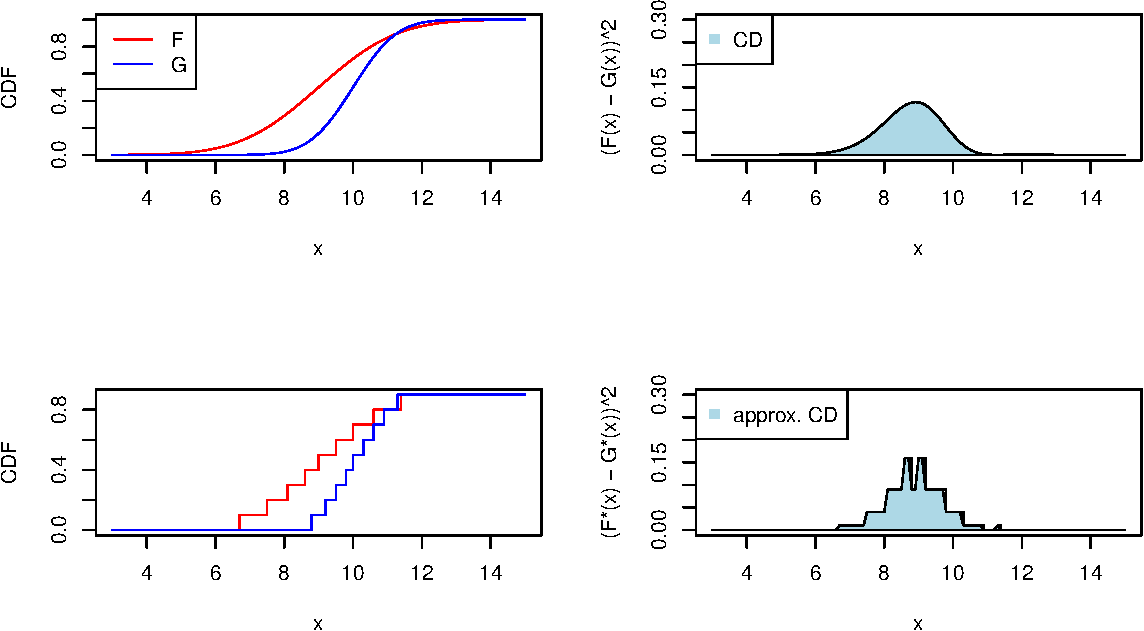
\includegraphics{cd_approx_2_files/figure-latex/unnamed-chunk-2-1.pdf}

In this example, six different approximations are applied to the
distributions \(F~N(9, 1.8)\) and \(G~N(10, 1)\) in the figures above.

\begin{itemize}
\tightlist
\item
  Using direct numerical integration based on a fine grid of values for
  \(x\):
\end{itemize}

\begin{verbatim}
## [1] 0.2532376
\end{verbatim}

\begin{itemize}
\tightlist
\item
  Using sampling and the alternative expression
  \eqref{eq:formulation_expectations} of the CD from above:
\end{itemize}

\begin{verbatim}
## [1] 0.2457156
\end{verbatim}

\begin{itemize}
\tightlist
\item
  Using the first quantile-based approximation \eqref{eq:approx2} and
  various values of \(K\):
\end{itemize}

\begin{verbatim}
## [1] 0.3550788 0.3078906 0.2764153 0.2652018 0.2593619 0.2557450 0.2545077
## [8] 0.2538792
\end{verbatim}

\begin{itemize}
\tightlist
\item
  Using the second quantile-based approximation \eqref{eq:approx2} and
  various values of \(K\):
\end{itemize}

\begin{verbatim}
## [1] 0.2926809 0.2723571 0.2608768 0.2572045 0.2552998 0.2541028 0.2536835
## [8] 0.2534662
\end{verbatim}

\begin{itemize}
\tightlist
\item
  Using the left-sided Riemann sum approximation and various values of
  \(K\):
\end{itemize}

\begin{verbatim}
## [1] 0.2370715 0.2458022 0.2505461 0.2520862 0.2527531 0.2530874 0.2531764
## [8] 0.2532128
\end{verbatim}

\begin{itemize}
\tightlist
\item
  Using the trapezoidal Riemann sum approximation and various values of
  \(K\):
\end{itemize}

\begin{verbatim}
## [1] 0.2854597 0.2575762 0.2543386 0.2552775 0.2540318 0.2535609 0.2534094
## [8] 0.2533309
\end{verbatim}

The below plot shows the results from the different computations.

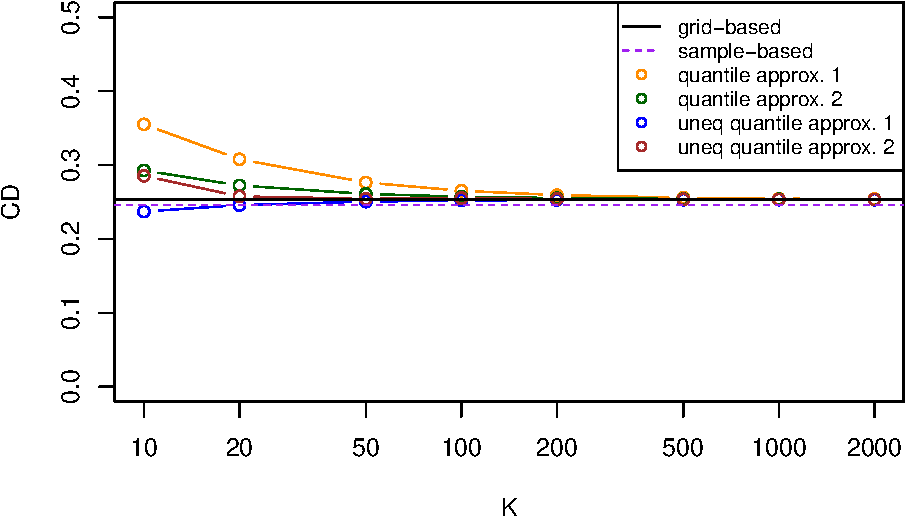
\includegraphics{cd_approx_2_files/figure-latex/unnamed-chunk-10-1.pdf}

In the case that \(G\) is a point mass at \(y=10\), approximation
\eqref{eq:approx1} indeed coincides with
\eqref{eq:linear_quantile_scores}.

\begin{verbatim}
## [1] "Quantile approx. 1: 0.688567227886639"
\end{verbatim}

\begin{verbatim}
## [1] "Quantile approx. 2: 0.608983067073759"
\end{verbatim}

\begin{verbatim}
## [1] "Uneq quantile approx. 1: 1.03814992169128"
\end{verbatim}

\begin{verbatim}
## [1] "Uneq quantile approx. 2: 1.24791020451193"
\end{verbatim}

\begin{verbatim}
## [1] "Quantile score WIS: 0.688567227886639"
\end{verbatim}

The approximation \eqref{eq:approx1} is closer to the grid-based direct
evaluation of the integral. Since the unequally-spaced approximations
were not formulated from (equally-spaced) WIS, it may be expected.

\begin{verbatim}
## [1] "Grid-based approx.: 0.61599852942592"
\end{verbatim}

\hypertarget{unequally-spaceed-intervals}{%
\subsection{Unequally-spaceed
intervals}\label{unequally-spaceed-intervals}}

We apply the same six approximations as in the previous example to the
two distributions \(F\sim N(8,2)\) and \(G \sim N(11,1)\) whose
quantiles correspond to unequally-spaced probability levels.

\hypertarget{quantiles-with-unequally-spaced-intervals}{%
\subsubsection{7 quantiles with unequally-spaced
intervals}\label{quantiles-with-unequally-spaced-intervals}}

The probability levels corresponding to the given set of quantiles in
this example is \(0.025,0.1,0.25,0.5,0.75,0.9,0.975\), which is the same
probability levels provided by the COVID-hub case forecasts.

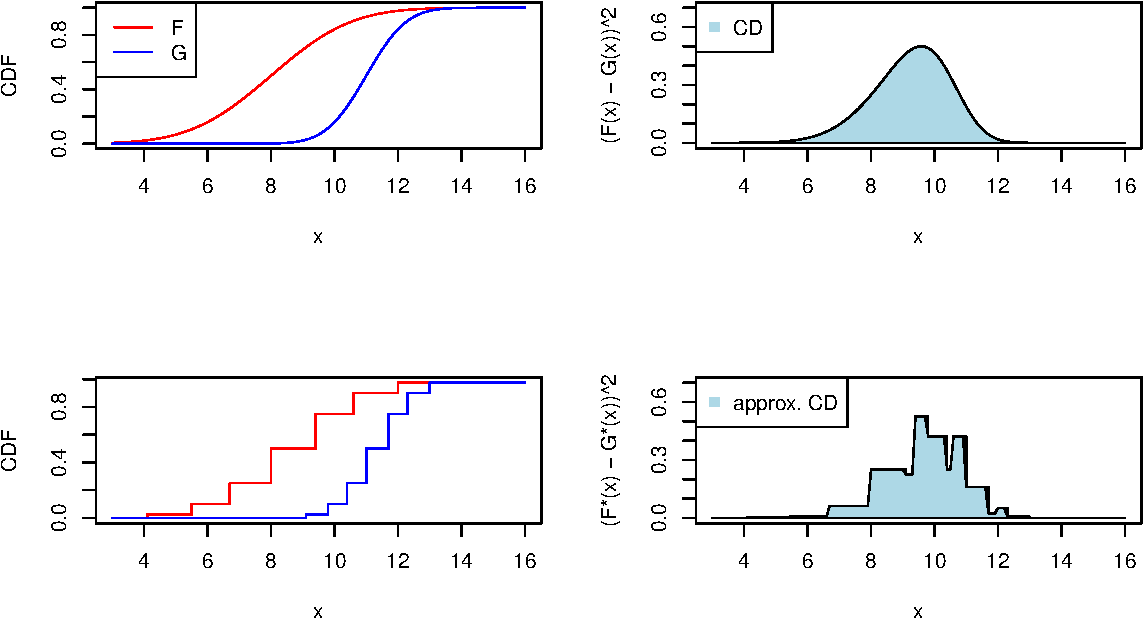
\includegraphics{cd_approx_2_files/figure-latex/unnamed-chunk-13-1.pdf}

\begin{itemize}
\tightlist
\item
  Using direct numerical integration based on a fine grid of values for
  \(x\).
\end{itemize}

\begin{verbatim}
## [1] 1.493653
\end{verbatim}

\begin{itemize}
\tightlist
\item
  Using sampling and the alternative expression
  \eqref{eq:formulation_expectations} of the CD from above:
\end{itemize}

\begin{verbatim}
## [1] 1.483948
\end{verbatim}

\begin{itemize}
\tightlist
\item
  Using the first quantile-based approximation:
\end{itemize}

\begin{verbatim}
## [1] 1.919252
\end{verbatim}

\begin{itemize}
\tightlist
\item
  Using the second quantile-based approximation:
\end{itemize}

\begin{verbatim}
## [1] 1.764859
\end{verbatim}

\begin{itemize}
\tightlist
\item
  Using the left-sided Riemann sum-based approximation:
\end{itemize}

\begin{verbatim}
## [1] 1.35122
\end{verbatim}

\begin{itemize}
\tightlist
\item
  Using the trapezoidal Riemann sum-based approximation:
\end{itemize}

\begin{verbatim}
## [1] 1.468801
\end{verbatim}

Out of all four quantile-based approximation, the trapezoidal Riemann
sum-based approximation is closest to the grid-based integral
evaluation.

\hypertarget{quantiles-with-2-unequally-spaced-probability-levels-at-the-tails}{%
\subsubsection{23 quantiles with 2 unequally-spaced probability levels
at the
tails}\label{quantiles-with-2-unequally-spaced-probability-levels-at-the-tails}}

Using the same \(F\) and \(G\), the probability levels corresponding to
the given set of quantiles in this example is the same probability
levels provided by the COVID-hub death forecasts. They are almost
equally-spaced, except at the tails.

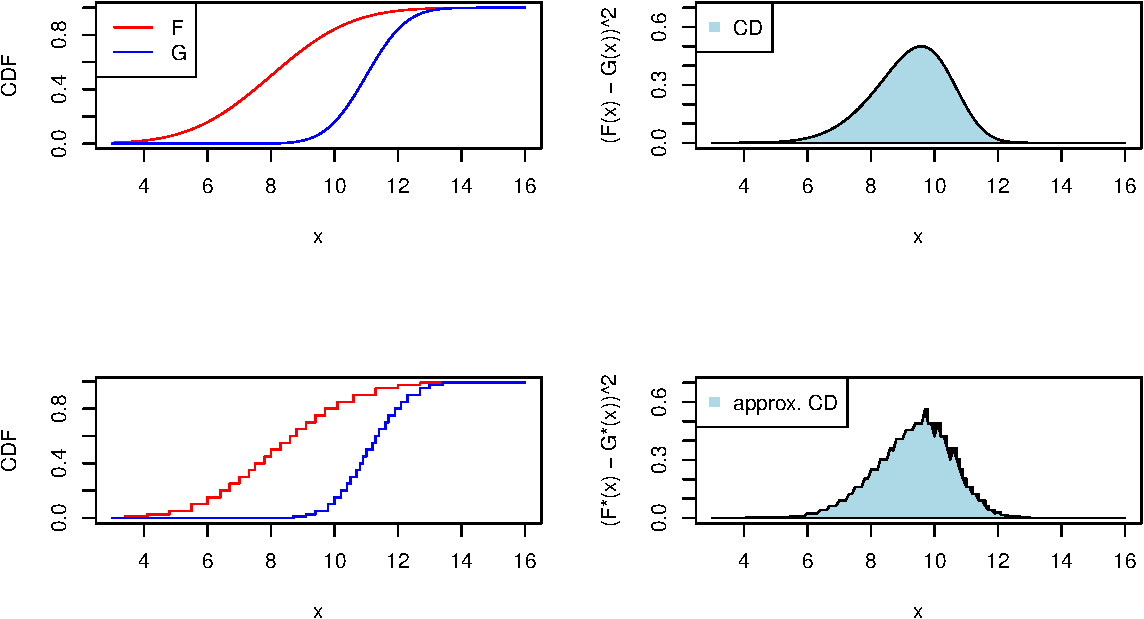
\includegraphics{cd_approx_2_files/figure-latex/unnamed-chunk-20-1.pdf}

\begin{itemize}
\tightlist
\item
  Using the first quantile-based approximation:
\end{itemize}

\begin{verbatim}
## [1] 1.640408
\end{verbatim}

\begin{itemize}
\tightlist
\item
  Using the second quantile-based approximation:
\end{itemize}

\begin{verbatim}
## [1] 1.581296
\end{verbatim}

\begin{itemize}
\tightlist
\item
  Using the left-sided Riemann sum-based approximation:
\end{itemize}

\begin{verbatim}
## [1] 1.452266
\end{verbatim}

\begin{itemize}
\tightlist
\item
  Using the trapezoidal Riemann sum-based approximation:
\end{itemize}

\begin{verbatim}
## [1] 1.470718
\end{verbatim}

Again, the trapezoidal Riemann sum-based approximation is closest to the
grid-based integral evaluation of 1.493653.

\hypertarget{examples-of-disagreement-between-equally--and-unequally-spaced-interval-methods}{%
\subsubsection{Examples of Disagreement Between Equally- and
Unequally-spaced Interval
Methods}\label{examples-of-disagreement-between-equally--and-unequally-spaced-interval-methods}}

\hypertarget{heavy-tails}{%
\paragraph{Heavy tails}\label{heavy-tails}}

Suppose we have three cumulative distributions, \(F\sim N(1,1)\),
\(G\sim N(2,1)\) and \(H\sim T_1\), represented by 7 unequally-spaced
quantiles. The probability levels corresponding to the given set of
quantiles in this example is \(0.025,0.1,0.25,0.5,0.75,0.9,0.975\).

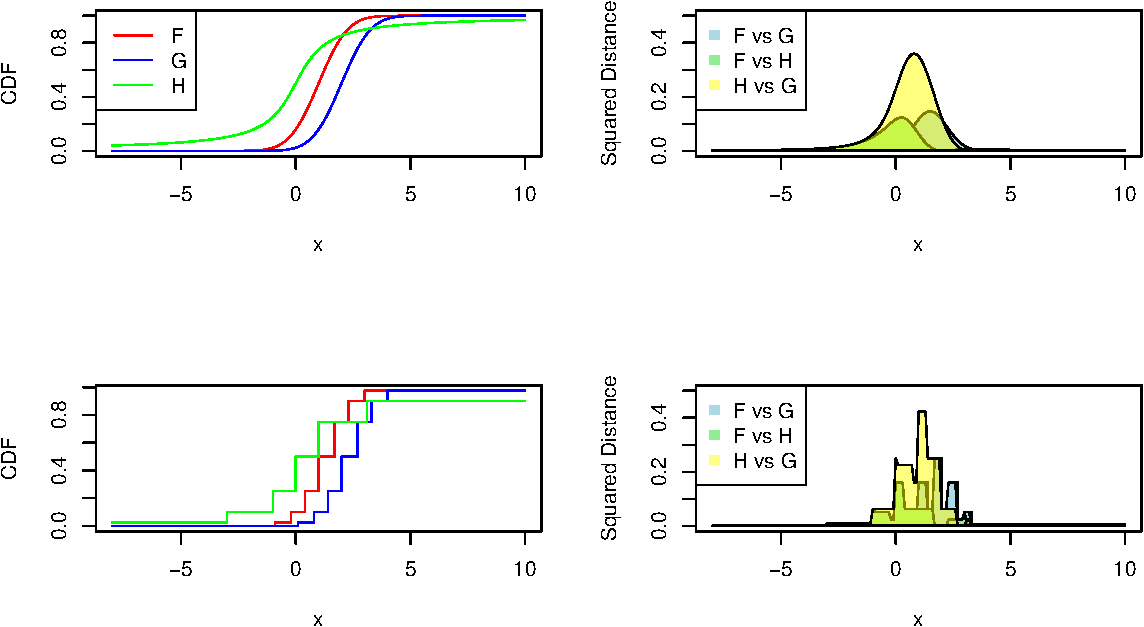
\includegraphics{cd_approx_2_files/figure-latex/unnamed-chunk-25-1.pdf}

\begin{itemize}
\tightlist
\item
  Using direct numerical integration based on a fine grid of values for
  \(x\).
\end{itemize}

\begin{verbatim}
## [1] "CD of F vs G: 0.270903289652979"
\end{verbatim}

\begin{verbatim}
## [1] "CD of F vs H: 0.303008857878541"
\end{verbatim}

\begin{verbatim}
## [1] "CD of H vs G: 0.830227986212452"
\end{verbatim}

\begin{itemize}
\tightlist
\item
  Using the first quantile-based approximation:
\end{itemize}

\begin{verbatim}
## [1] "Approx. CD of F vs G: 0.430834455349389"
\end{verbatim}

\begin{verbatim}
## [1] "Approx. CD of F vs H: 0.412836097817344"
\end{verbatim}

\begin{verbatim}
## [1] " Approx. CD of H vs G: 1.0891147790307"
\end{verbatim}

\begin{itemize}
\tightlist
\item
  Using the second quantile-based approximation:
\end{itemize}

\begin{verbatim}
## [1] "Approx. CD of F vs G: 0.349525091827873"
\end{verbatim}

\begin{verbatim}
## [1] "Approx. CD of F vs H: 0.318185573750552"
\end{verbatim}

\begin{verbatim}
## [1] " Approx. CD of H vs G: 0.958988318892232"
\end{verbatim}

\begin{itemize}
\tightlist
\item
  Using the left-sided Riemann sum-based approximation:
\end{itemize}

\begin{verbatim}
## [1] "Approx. CD of F vs G: 0.267605148430715"
\end{verbatim}

\begin{verbatim}
## [1] "Approx. CD of F vs H: 0.243610829902767"
\end{verbatim}

\begin{verbatim}
## [1] " Approx. CD of H vs G: 0.734225431651865"
\end{verbatim}

\begin{itemize}
\tightlist
\item
  Using the trapezoidal Riemann sum-based approximation:
\end{itemize}

\begin{verbatim}
## [1] "Approx. CD of F vs G: 0.302511061162121"
\end{verbatim}

\begin{verbatim}
## [1] "Approx. CD of F vs H: 0.266926890705267"
\end{verbatim}

\begin{verbatim}
## [1] " Approx. CD of H vs G: 0.752143988834321"
\end{verbatim}

\hypertarget{long-tails}{%
\paragraph{Long tails}\label{long-tails}}

Suppose we have three cumulative distributions, \(F\sim N(0,1)\),
\(G\sim N(1,1)\) and \(H\sim \text{Laplace}(0,1)\), represented by 7
unequally-spaced quantiles. The probability levels corresponding to the
given set of quantiles in this example is
\(0.025,0.1,0.25,0.5,0.75,0.9,0.975\).

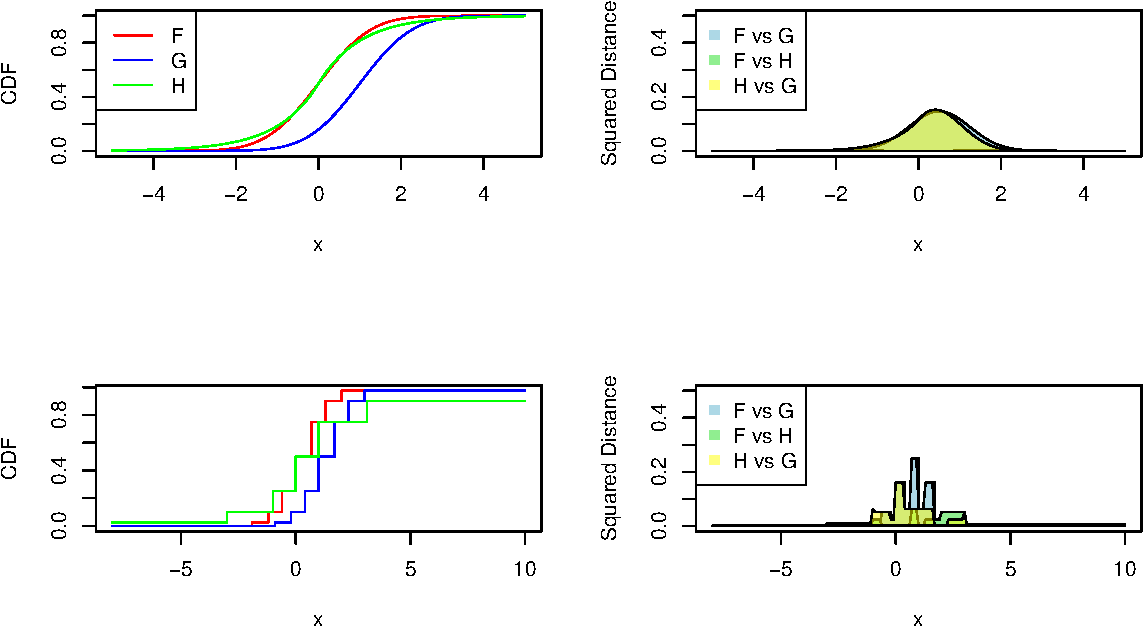
\includegraphics{cd_approx_2_files/figure-latex/unnamed-chunk-31-1.pdf}

\begin{itemize}
\tightlist
\item
  Using direct numerical integration based on a fine grid of values for
  \(x\).
\end{itemize}

\begin{verbatim}
## [1] "CD of F vs G: 0.270903289581517"
\end{verbatim}

\begin{verbatim}
## [1] "CD of F vs H: 0.0068412250422997"
\end{verbatim}

\begin{verbatim}
## [1] "CD of H vs G: 0.257655267503305"
\end{verbatim}

\begin{itemize}
\tightlist
\item
  Using the first quantile-based approximation:
\end{itemize}

\begin{verbatim}
## [1] "Approx. CD of F vs G: 0.430834455349389"
\end{verbatim}

\begin{verbatim}
## [1] "Approx. CD of F vs H: 0.0203971216157386"
\end{verbatim}

\begin{verbatim}
## [1] " Approx. CD of H vs G: 0.416591384312851"
\end{verbatim}

\begin{itemize}
\tightlist
\item
  Using the second quantile-based approximation:
\end{itemize}

\begin{verbatim}
## [1] "Approx. CD of F vs G: 0.349525091827873"
\end{verbatim}

\begin{verbatim}
## [1] "Approx. CD of F vs H: 0.0116554980661363"
\end{verbatim}

\begin{verbatim}
## [1] " Approx. CD of H vs G: 0.333247296357544"
\end{verbatim}

\begin{itemize}
\tightlist
\item
  Using the left-sided Riemann sum-based approximation:
\end{itemize}

\begin{verbatim}
## [1] "Approx. CD of F vs G: 0.267605148430715"
\end{verbatim}

\begin{verbatim}
## [1] "Approx. CD of F vs H: 0.00892374070688564"
\end{verbatim}

\begin{verbatim}
## [1] " Approx. CD of H vs G: 0.255142461273745"
\end{verbatim}

\begin{itemize}
\tightlist
\item
  Using the trapezoidal Riemann sum-based approximation:
\end{itemize}

\begin{verbatim}
## [1] "Approx. CD of F vs G: 0.302511061162121"
\end{verbatim}

\begin{verbatim}
## [1] "Approx. CD of F vs H: 0.0194133332014688"
\end{verbatim}

\begin{verbatim}
## [1] " Approx. CD of H vs G: 0.259617817413175"
\end{verbatim}

\end{document}
